% questions.tex —— 2007 年·普通高等学校招生考试·重庆卷·文科 · 题目内容片段（无答案）
% 由 tools/generate_projects.py 依来源总账自 2007/2007_数学真题_重庆文_试题.md 生成，勿手改（改源 MD 后重跑）


状态：needs-review；依固定候选 PDF 两页（印刷页 357–358）三栏图像以 300 dpi 渲染逐题核验，图形已矢量重绘，正式构建与逐页验收待完成。源未列各题分值，不补分值。

\gkpart{一、选择题}

\begin{question}
\gkti{1}在等比数列 $\{a_n\}$ 中，$a_2=8$，$a_1=64$，则公比 $q$ 为（　）

（A）$2$

（B）$3$

（C）$4$

（D）$8$

\end{question}
\begin{question}
\gkti{2}设全集 $U=\{a,b,c,d\}$，$A=\{a,c\}$，$B=\{b\}$，则 $A\cap(\complement_UB)=$（　）

（A）$\varnothing$

（B）$\{a\}$

（C）$\{c\}$

（D）$\{a,c\}$

\end{question}
\begin{question}
\gkti{3}垂直于同一平面的两条直线（　）

（A）平行

（B）垂直

（C）相交

（D）异面

\end{question}
\begin{question}
\gkti{4}$(2x-1)^6$ 展开式中 $x^2$ 的系数为（　）

（A）$15$

（B）$60$

（C）$120$

（D）$240$

\end{question}
\begin{question}
\gkti{5}“$-1<x<1$”是“$x^2<1$”的（　）

（A）充分必要条件

（B）充分但不必要条件

（C）必要但不充分条件

（D）既不充分也不必要条件

\end{question}
\begin{question}
\gkti{6}下列各式中，值为 $\dfrac{\sqrt3}{2}$ 的是（　）

（A）$2\sin15^\circ\cos15^\circ$

（B）$\cos^215^\circ-\sin^215^\circ$

（C）$2\sin^215^\circ-1$

（D）$\sin^215^\circ+\cos^215^\circ$

\end{question}
\begin{question}
\gkti{7}从 $5$ 张 $100$ 元，$3$ 张 $200$ 元，$2$ 张 $300$ 元的奥运预赛门票中任取 $3$ 张，则所取 $3$ 张中至少有 $2$ 张价格相同的概率为（　）

（A）$\dfrac14$

（B）$\dfrac{79}{120}$

（C）$\dfrac34$

（D）$\dfrac{23}{24}$

\end{question}
\begin{question}
\gkti{8}若直线 $y=kx+1$ 与圆 $x^2+y^2=1$ 相交于 $P$，$Q$ 两点，且 $\angle POQ=120^\circ$（其中 $O$ 为原点），则 $k$ 的值为（　）

（A）$-\sqrt3$ 或 $\sqrt3$

（B）$\sqrt3$

（C）$-\sqrt2$ 或 $\sqrt2$

（D）$\sqrt2$

\end{question}
\begin{question}
\gkti{9}已知向量 $\overrightarrow{OA}=(4,6)$，$\overrightarrow{OB}=(3,5)$，且 $\overrightarrow{OC}\perp\overrightarrow{OA}$，$\overrightarrow{AC}\parallel\overrightarrow{OB}$，则向量 $\overrightarrow{OC}=$（　）

（A）$\left(-\dfrac37,\dfrac27\right)$

（B）$\left(-\dfrac27,\dfrac4{21}\right)$

（C）$\left(\dfrac37,-\dfrac27\right)$

（D）$\left(\dfrac27,-\dfrac4{21}\right)$

\end{question}
\begin{question}
\gkti{10}设 $P(3,1)$ 为二次函数 $f(x)=ax^2-2ax+b$（$x\geqslant1$）的图象与其反函数 $y=f^{-1}(x)$ 的图象的一个交点，则（　）

（A）$a=\dfrac12$，$b=\dfrac52$

（B）$a=\dfrac12$，$b=-\dfrac52$

（C）$a=-\dfrac12$，$b=\dfrac52$

（D）$a=-\dfrac12$，$b=-\dfrac52$

\end{question}
\begin{question}
\gkti{11}设 $\sqrt3b$ 是 $1-a$ 和 $1+a$ 的等比中项，则 $a+3b$ 的最大值为（　）

（A）$1$

（B）$2$

（C）$3$

（D）$4$

\end{question}
\begin{question}
\gkti{12}已知以 $F_1(-2,0)$，$F_2(2,0)$ 为焦点的椭圆与直线 $x+\sqrt3y+4=0$ 有且仅有一个交点，则椭圆的长轴长为（　）

（A）$3\sqrt2$

（B）$2\sqrt6$

（C）$2\sqrt7$

（D）$4\sqrt2$

\end{question}
\gkpart{二、填空题}

\begin{question}
\gkti{13}在 $\triangle ABC$ 中，$AB=1$，$BC=2$，$B=60^\circ$，则 $AC=$\gkblank{}。

\end{question}
\begin{question}
\gkti{14}已知 $\begin{cases}2x+3y\leqslant6,\\ x-y\geqslant0,\\ y\geqslant0,\end{cases}$ 则 $z=3x-y$ 的最大值为\gkblank{}。

\end{question}
\begin{question}
\gkti{15}要排出某班一天中语文、数学、政治、英语、体育、艺术 $6$ 门课各一节的课程表，要求数学课排在前 $3$ 节，英语课不排在第 $6$ 节，则不同的排法种数为\gkblank{}。（以数字作答）

\end{question}
\begin{question}
\gkti{16}函数 $f(x)=\sqrt{x^2-2x}+2\sqrt{x^2-5x+4}$ 的最小值为\gkblank{}。

\end{question}
\gkpart{三、解答题}

\begin{question}
\gkti{17}设甲、乙两人每次射击命中目标的概率分别为 $\dfrac34$ 和 $\dfrac45$，且各次射击相互独立。

（1）若甲、乙各射击一次，求甲命中但乙未命中目标的概率；

（2）若甲、乙各射击两次，求两人命中目标的次数相等的概率。

\end{question}
\begin{question}
\gkti{18}已知函数 $f(x)=\dfrac{1+\sqrt2\cos\left(2x-\dfrac{\pi}{4}\right)}{\sin\left(x+\dfrac{\pi}{2}\right)}$。

（1）求 $f(x)$ 的定义域；

（2）若角 $\alpha$ 在第一象限且 $\cos\alpha=\dfrac35$，求 $f(\alpha)$。

\Needspace{0.4\textheight}
\end{question}
\begin{question}
\gkti{19}如图，在直三棱柱 $ABC-A_1B_1C_1$ 中，$\angle ABC=90^\circ$，$AB=1$，$BC=\dfrac32$，$AA_1=2$；点 $D$ 在棱 $BB_1$ 上，$BD=\dfrac13BB_1$；$B_1E\perp A_1D$，垂足为 $E$。求：

（1）异面直线 $A_1D$ 与 $B_1C_1$ 的距离；

（2）四棱锥 $C-ABDE$ 的体积。
\nopagebreak[4]
\begin{center}% 2007 年重庆卷文科第 19 题：直三棱柱 ABC-A1B1C1，∠ABC=90°，AB=1，BC=3/2，AA1=2；
%   D 在 BB1 上且 BD=BB1/3，B1E⊥A1D 于 E。图中 E 位于 A1D 上、B1 的左下方。
% 来源 PDF：gaokaomath-src/普通高考/2007/2007重庆文.pdf
% SHA-256：a647b60227db10d70c5c3fbe72b6ffe2c8a0667b233695e55bb4f5a7cef633a6
% 原页：2007重庆文.pdf 第 1 页（A3 三栏）第 3 栏，书页码 357。
% 重绘依据：按原页 A1、C1、B1、E、D、A、B、C 的相对位置与虚实线重绘；
%   斜投影的深度偏移取 0.55，使 D（BB1 的三分之一处）与底面对角线 AC 在图上分开。
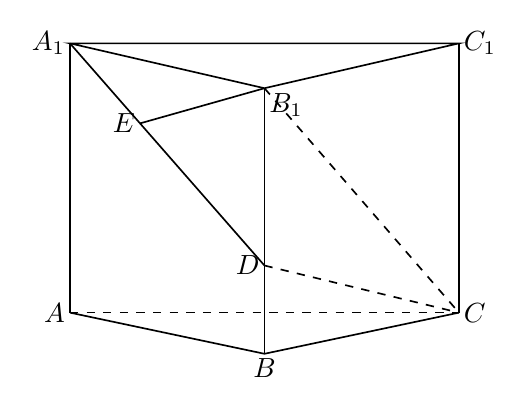
\begin{tikzpicture}[scale=0.95, semithick,
  every node/.style={inner sep=1.5pt}]

  \coordinate (A)  at (0.0,0.55);
  \coordinate (B)  at (2.60,0.00);
  \coordinate (C)  at (5.20,0.55);
  \coordinate (A1) at (0.0,4.15);
  \coordinate (B1) at (2.60,3.55);
  \coordinate (C1) at (5.20,4.15);
  \coordinate (D)  at (2.60,1.18);
  \coordinate (E)  at (0.936,3.08);

  % 底面
  \draw (A) -- (B) -- (C);
  \draw[dashed] (A) -- (C);
  % 侧棱
  \draw (A) -- (A1);
  \draw (B) -- (B1);
  \draw (C) -- (C1);
  % 上底面
  \draw (A1) -- (B1) -- (C1) -- cycle;

  % 题设连线
  \draw (A1) -- (D);
  \draw (B1) -- (E);
  \draw[dashed] (B1) -- (C);
  \draw[dashed] (D) -- (C);

  \node[left] at (A) {$A$};
  \node[below] at (B) {$B$};
  \node[right] at (C) {$C$};
  \node[left] at (A1) {$A_1$};
  \node[below right] at (B1) {$B_1$};
  \node[right] at (C1) {$C_1$};
  \node[left] at (D) {$D$};
  \node[left] at (E) {$E$};
\end{tikzpicture}
\end{center}
\nopagebreak[4]
\end{question}
\begin{question}
\gkti{20}用长为 $18\ \mathrm m$ 的钢条围成一个长方体形状的框架，要求长方体的长与宽之比为 $2:1$，问该长方体的长、宽、高各为多少时，其体积最大？最大体积是多少？

\Needspace{0.4\textheight}
\end{question}
\begin{question}
\gkti{21}如图，倾斜角为 $\alpha$ 的直线经过抛物线 $y^2=8x$ 的焦点 $F$，且与抛物线交于 $A$、$B$ 两点。

（1）求抛物线的焦点 $F$ 的坐标及准线 $l$ 方程；

（2）若 $\alpha$ 为锐角，作线段 $AB$ 的垂直平分线 $m$ 交 $x$ 轴于点 $P$，证明 $|FP|-|FP|\cos2\alpha$ 为定值，并求此定值。
\nopagebreak[4]
\begin{center}% 2007 年重庆卷文科第 21 题：抛物线 y^2=8x、焦点 F、准线 l 与过 F 的直线交于 A、B；
%   弦 AB 的垂直平分线 m 交 x 轴于 P，倾斜角 α 标在直线与 x 轴之间。
% 来源 PDF：gaokaomath-src/普通高考/2007/2007重庆文.pdf
% SHA-256：a647b60227db10d70c5c3fbe72b6ffe2c8a0667b233695e55bb4f5a7cef633a6
% 原页：2007重庆文.pdf 第 2 页（A3 三栏）第 2 栏，书页码 358。
% 重绘依据：按 α=60° 作图（A 在上、B 在下、P 在焦点右侧）；m 取过弦中点 M(10/3,2√3)、
%   斜率 −1/√3 的直线，与 x 轴的交点即 P(22/3,0)，与原页位置关系一致。
\begin{tikzpicture}[x=0.78cm, y=0.52cm, semithick,
  every node/.style={inner sep=1.5pt}]

  % 坐标轴
  \draw[->,>=stealth] (-2.8,0) -- (8.6,0) node[right] {$x$};
  \draw[->,>=stealth] (0,-7.6) -- (0,8.2) node[above] {$y$};
  \node[below left] at (0,0) {$O$};

  % 准线 l：x=-2
  \draw (-2,-7.2) -- (-2,7.6) node[above] {$l$};

  % 抛物线 y^2=8x
  \draw[domain=-7.2:7.2,samples=160,line width=1pt] plot ({\x*\x/8},{\x});

  % 过 F 的直线（α=60°），交抛物线于 A、B
  \coordinate (F) at (2,0);
  \coordinate (A) at (6,6.928);
  \coordinate (B) at (0.667,-2.309);
  \draw (B) -- (A);

  % 弦 AB 的垂直平分线 m（过中点 M，斜率 -1/√3），交 x 轴于 P
  \coordinate (P) at (7.333,0);
  \draw (1.2,3.539) -- (8.3,-0.559);
  \node[above left] at (1.2,3.539) {$m$};

  % 角 α
  \draw (2.9,0) arc[start angle=0,end angle=60,radius=0.9];
  \node at (3.35,0.95) {$\alpha$};

  \fill (F) circle (1.3pt);
  \fill (P) circle (1.3pt);
  \node[below right=2pt] at (F) {$F$};
  \node[below=3pt] at (P) {$P$};
  \node[above left] at (A) {$A$};
  \node[below left] at (B) {$B$};
\end{tikzpicture}
\end{center}
\nopagebreak[4]
\end{question}
\begin{question}
\gkti{22}已知各项均为正数的数列 $\{a_n\}$ 的前 $n$ 项和 $S_n$ 满足 $S_1>1$，且 $6S_n=(a_n+1)(a_n+2)$，$n\in\mathbf N_+$。

（1）求 $\{a_n\}$ 的通项公式；

（2）设数列 $\{b_n\}$ 满足 $a_n(2^{b_n}-1)=1$，并记 $T_n$ 为 $\{b_n\}$ 的前 $n$ 项和，求证：$3T_n+1>\log_2(a_n+3)$，$n\in\mathbf N_+$。

\end{question}